\documentclass[11pt]{article}

\usepackage{url}
\usepackage{multicol}
\usepackage[english]{babel}
\usepackage[margin=1in]{geometry}
\usepackage{graphicx}
\usepackage{subcaption}
\usepackage{enumitem}
\usepackage{amsmath}
\usepackage{amssymb}
\usepackage{wasysym}
\usepackage{color}
\usepackage{float}
\usepackage{nomencl}
\usepackage[title]{appendix}
\makenomenclature
\usepackage{pdfpages}
\usepackage{algorithm}
\usepackage{algpseudocode}
\usepackage{hyperref}
\hypersetup{
    colorlinks=true,
    linkcolor=blue,
    filecolor=magenta,      
    urlcolor=cyan,
    pdftitle={Overleaf Example},
    pdfpagemode=FullScreen,
    }
\title{16-745 Optimal Control Lecture 13}
\author{Reid Graves} 

\begin{document}
\maketitle

\section*{Last Time:}
\begin{itemize}
    \item DDP details
    \item Constraints
\end{itemize}

\section*{Today} 
Other domain of nonlinear control- Direct methods. (Before did indirect/shooting). Indirect optimizes first, then discretizes. Direct discretizes first, then optimizes.
\begin{itemize}
    \item Minimum / Free-Time problems
    \item Direct Trajectory Optimization
    \item Direct Collocation
    \item Sequential Quadratic Programming
\end{itemize}

\section*{Handling Free / Minimum-Time Problems}

free time- instead of defining time horizon, let the controller figure it out. The Minimum time problem is:

\begin{equation*}
    \min_{x(t), u(t), T_f} \quad J = \int_0^{T_f} 1 \, dt
\end{equation*}

subject to:

\begin{equation*}
    \dot{x} = f(x, u)
\end{equation*}

Add goal constraint- need to get to goal:
\begin{equation*}
    x(T_f) = x_{\text{goal}}
\end{equation*}

Add input constraints to ensure well posed.
\begin{equation*}
    u_{\min} \leq u(t) \leq u_{\max}
\end{equation*}


\begin{itemize}
    \item We don't want to change the number of knot points. So change length of each timestep instead of number of knot points.
    \item Make $h$ (time step) from RK a control input:
    
    \begin{equation*}
        x_{k+1} = f_{\text{RK4}}(x_k, \bar{u}_k), \quad \bar{u}_k = \begin{bmatrix} u_k \\ h_k \end{bmatrix}
    \end{equation*}
    
    \item Also want to scale the cost by $h$, e.g.,
    
    \begin{equation*}
        {J}(x, u) = \sum_{u=1}^{k} h_k l(x_k, u_k) + l_N(x_N)
    \end{equation*}
    \item Requires constraints on $h$. Otherwise, the solver can ``cheat physics'' by making $h$ very large or negative to exploit discretization errors.
    \item Always nonlinear/nonconvex, even if the dynamics are linear. $h$ is multiplying the dynamics, so get quadratic terms in dynamics, making problem nonlinear.
\end{itemize}

\section*{Direct Trajectory Optimization}

\begin{itemize}
    \item \textbf{Basic strategy:} Discretize / ``transcribe'' continuous-time optimal control problem into a standard nonlinear program (NLP):

    \textcolor{blue}{\textbf{``Standard" NLP}}
    
    \begin{equation*}
        \begin{aligned}
            &\min_{x} \quad f(x) \quad \textcolor{blue}{\text{(cost function)}} \\
            &\text{s.t.} \quad c(x) = 0 \quad \textcolor{blue}{\text{(dynamics constraints)}} \\
            &\hspace{10mm} d(x) \leq 0 \quad \textcolor{blue}{\text{(other constraints- actuator limits, etc)}}
        \end{aligned}
    \end{equation*}

    \item All functions ($f,c,d$) assumed $C^2$ smooth.
    \item Lots of off-the-shelf solvers for large-scale NLP.
    \item Most common:
    \begin{itemize}
        \item IPOPT (free)
        \item SNOPT (commercial)
        \item KNITRO (commercial)
    \end{itemize}
    \item Common solution strategy: Sequential Quadratic Programming (SQP)-this is what SNOPT does. Also most common technique for nonlinear MPC.
\end{itemize}

\section*{SQP: Sequential Quadratic Programming}

\begin{itemize}
    \item \textbf{Strategy:} use 2\textsuperscript{nd}-order Taylor expansion of the Lagrangian and linearize $c(x)$, $d(x)$ to approximate the NLP as a QP:

    \begin{equation*}
        \min_{\Delta x} \quad f(x) + g^T \Delta x + \frac{1}{2} \Delta x^T H \Delta x
    \end{equation*}
    
    subject to:
    
    \begin{equation*}
        C(x) + C \Delta x = 0
    \end{equation*}
    
    \begin{equation*}
        d(x) + D \Delta x \leq 0
    \end{equation*}
    
    where:
    
    \begin{equation*}
        H = \frac{\partial^2 L}{\partial x^2}, \quad g = \frac{\partial L}{\partial x}, \quad C = \frac{\partial C}{\partial x}, \quad D = \frac{\partial d}{\partial x}
    \end{equation*}

    \begin{equation*}
        L(x, \lambda, \mu) = f(x) + \lambda^T c(x) + \mu^T d(x)
    \end{equation*}

    \item Solve QP to compute primal-dual search direction:
    
    \begin{equation*}
        \Delta z =
        \begin{bmatrix}
            \Delta x \\
            \Delta \lambda \\
            \Delta \mu
        \end{bmatrix}
    \end{equation*}

    \item Perform line search with merit function.
    \item With only equality constraints, reduces to Newton’s method on KKT conditions:
    
    \begin{equation*}
        \underbrace{
        \begin{bmatrix}
            H & C^T \\
            C & 0
        \end{bmatrix}
        }_{\text{\textcolor{blue}{KKT System}}}
        \begin{bmatrix}
            \Delta x \\
            \Delta \lambda
        \end{bmatrix}
        =
        \begin{bmatrix}
            -g \\
            -c(x)
        \end{bmatrix}
    \end{equation*}
    \item Think of SQP as a generalization of Newton’s method to handle \textbf{inequalities}.
    \item Can use any QP solver for sub-problems, but good implementations typically warm start using the previous QP iteration.
    \item For good performance on trajectory optimization problems, taking advantage of sparsity in KKT systems is crucial.
    \item If inequalities are convex (e.g., conic), we can generalize SQP to \textbf{SCP} (Sequential Convex Programming), where inequalities are passed directly to the sub-problem solver.
    \item SCP is still an active research area.
\end{itemize}

\section*{Direct Collocation}

Direct collocation is gold standard direct method.

\begin{itemize}
    \item So far, we've used explicit \textbf{RK} methods:

    \begin{equation*}
        \dot{x} = f(x, u) \quad \Rightarrow \quad x_{k+1} = f(x_k, u_k)
    \end{equation*}

    \item This makes sense if you're doing rollout.
    \item However, in a direct method, we’re just enforcing dynamics as \textbf{equality constraints} between knot points:

    \begin{equation*}
        C_k(x_k, u_k, x_{k+1}, u_{k+1}) = 0
    \end{equation*}

    \item $\Rightarrow$ Implicit integration is ``free'' in this formulation.

    \item Collocation methods use polynomial splines to represent trajectories and enforce dynamics as constraints on spline derivatives
    \item Classic \textbf{DIRCOL} algorithm uses cubic splines for states and piecewise linear interpolation for $u(t)$.
    \item Very high-order polynomials are sometimes used (e.g., spacecraft trajectories), but this is not common.
    \item \textbf{DIRCOL Spline Approximations:}
% Insert figure here
\begin{figure}[H]
    \centering
    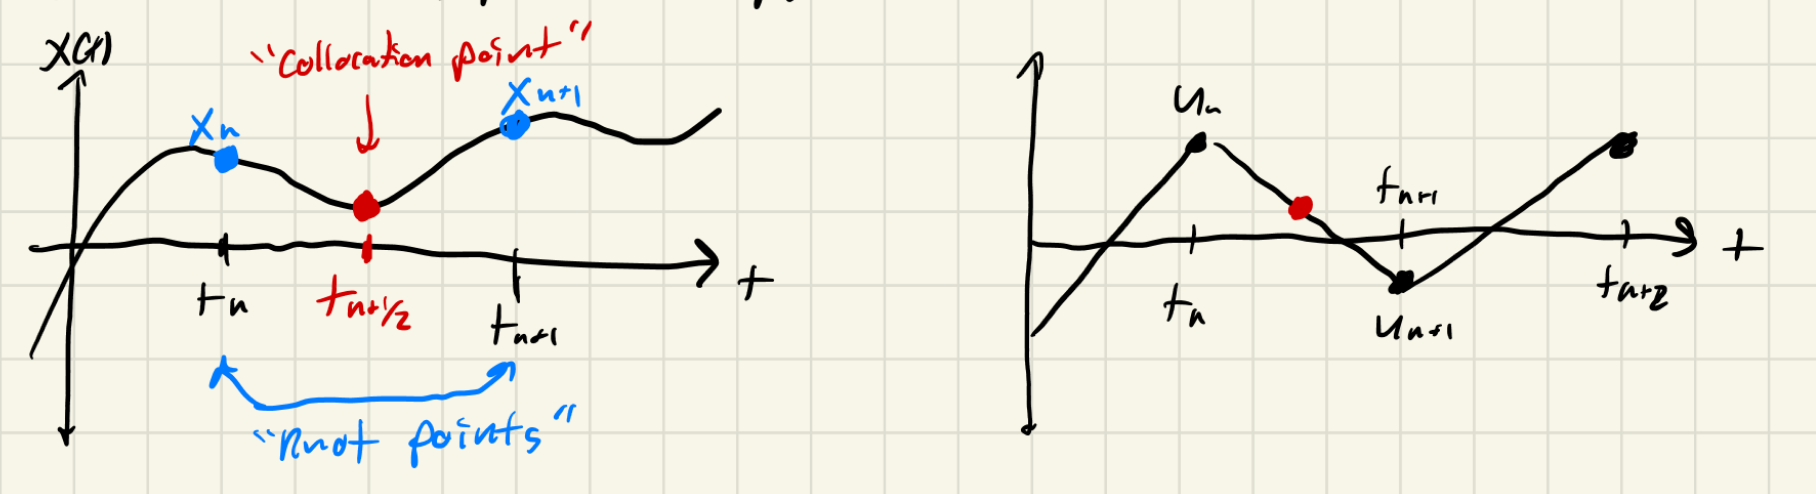
\includegraphics[width=0.95\linewidth]{lecture_13_1.png}
\end{figure}
    \begin{equation*}
    x(t) = C_0 + C_1 t + C_2 t^2 + C_3 t^3
\end{equation*}

\begin{equation*}
    \dot{x}(t) = C_1 + 2C_2 t + 3C_3 t^2
\end{equation*}

\subsection*{Matrix Formulation}

\begin{equation*}
    \begin{bmatrix}
        1 & 0 & 0 & 0 \\
        0 & 1 & 0 & 0 \\
        1 & h & h^2 & h^3 \\
        0 & 1 & 2h & 3h^2
    \end{bmatrix}
    \begin{bmatrix}
        C_0 \\ C_1 \\ C_2 \\ C_3
    \end{bmatrix}
    =
    \begin{bmatrix}
        x_k \\ \dot{x}_k \\ x_{k+1} \\ \dot{x}_{k+1}
    \end{bmatrix}
\end{equation*}

\subsection*{Inverted System}

\begin{equation*}
    \begin{bmatrix}
        1 & 0 & 0 & 0 \\
        0 & 1 & 0 & 0 \\
        -\frac{3}{h^2} & -\frac{2}{h} & \frac{3}{h^2} & -\frac{1}{h} \\
        \frac{2}{h^3} & \frac{1}{h^2} & -\frac{2}{h^3} & \frac{1}{h^2}
    \end{bmatrix}
    \begin{bmatrix}
        x_k \\ \dot{x}_k \\ x_{k+1} \\ \dot{x}_{k+1}
    \end{bmatrix}
    =
    \begin{bmatrix}
        C_0 \\ C_1 \\ C_2 \\ C_3
    \end{bmatrix}
\end{equation*}
\item{Evaluate at $t_{k+\frac{1}{2}}$}

\begin{equation*}
    x_{k+\frac{1}{2}} = x(t_k + \frac{h}{2}) = \frac{1}{2} (x_k + x_{k+1}) + \frac{h}{8} (\dot{x}_k - \dot{x}_{k+1})
\end{equation*}

\begin{align*}
   & = \frac{1}{2} (x_k + x_{k+1}) + \frac{h}{8} \big( f(x_k, u_k) - f(x_{k+1}, u_{k+1}) \big)
    \\
    &\hspace{40mm}\uparrow \hspace{20mm}\uparrow
\\
&\hspace{30mm}\textcolor{red}{\textit{(Continuous-time dynamics)}}
\end{align*}


\begin{equation*}
    \dot{x}_{k+\frac{1}{2}} = \dot{x}(t_k + \frac{h}{2}) = -\frac{3}{2h} (x_k - x_{k+1}) - \frac{1}{4} (\dot{x}_k + \dot{x}_{k+1})
\end{equation*}

\begin{equation*}
    = -\frac{3}{2h} (x_k - x_{k+1}) - \frac{1}{4} \big( f(x_k, u_k) + f(x_{k+1}, u_{k+1}) \big)
\end{equation*}

\begin{equation*}
    u_{k+\frac{1}{2}} = u(t_k + \frac{h}{2}) = \frac{1}{2} (u_k + u_{k+1})
\end{equation*}

\item{We can enforce Dynamics Constraints}

\begin{equation*}
    C_i (x_k, u_k, x_{k+1}, u_{k+1}) =
\end{equation*}

\begin{align*}
    &f(x_{k+\frac{1}{2}}, u_{k+\frac{1}{2}}) - \left[ -\frac{3}{2h} (x_k - x_{k+1}) - \frac{1}{4} \big( f(x_k, u_k) + f(x_{k+1}, u_{k+1}) \big) \right] = 0\\
   &\hspace{10mm} \uparrow\\
&\textcolor{blue}{\textit{(Continuous dynamics)}}
\end{align*}



    \item Note that only $x_k, u_k$ are decision variables (not $x_{k+\frac{1}{2}}, u_{k+\frac{1}{2}}$).
    \item Called \textbf{``Hermite-Simpson'' integration}.
    \item Achieves \textbf{3\textsuperscript{rd} order} integration accuracy like RK3.
    \item Requires \textbf{fewer dynamics calls} than explicit RK3!

\end{itemize}



\section*{Explicit RK3}

\begin{equation*}
    f_1 = f(x_k, u_k)
\end{equation*}

\begin{equation*}
    f_2 = f(x_k + \frac{1}{2} h f_1, u_k)
\end{equation*}

\begin{equation*}
    f_3 = f(x_k + 2h f_1 - h f_2, u_k)
\end{equation*}

\begin{equation*}
    x_{k+1} = x_k + \frac{h}{6} (f_1 + 4 f_2 + f_3)
\end{equation*}

$\Rightarrow$ \textbf{3 dynamics evaluations per time step}

\section*{Hermite-Simpson Integration}

\begin{equation*}
    f(x_{k+\frac{1}{2}}, u_{k+\frac{1}{2}}) + \frac{3}{2h} (x_k - x_{k+1})
\end{equation*}

\begin{align*}
    &- \frac{1}{4} \big( f(x_k, u_k) + f(x_{k+1}, u_{k+1}) \big) = 0 
    \\
    &\hspace{15mm}\uparrow \hspace{20mm}\uparrow
    \\
&\hspace{10mm}\textcolor{blue}{\textit{These get re-used at adjacent steps!}}
\end{align*}


$\Rightarrow$ \textbf{Only 2 dynamics calls per time step!}

\begin{itemize}
    \item Since dynamics calls often dominate total compute cost, this results in a \textbf{$\sim$50\% savings}.
\end{itemize}

\section*{Example}

\begin{itemize}
    \item Acrobot with \textbf{DIRCOL}
    \item Warm-starting with dynamically infeasible guesses can help a lot!
\end{itemize}

\end{document}
